\documentclass[10pt]{article}

\usepackage[utf8]{inputenc} % Required for inputting international characters
\usepackage[T1]{fontenc} % Output font encoding for international characters
\usepackage[tocflat]{tocstyle}
\usetocstyle{standard}
\usepackage{blindtext}
\usepackage{mathpazo} % Palatino font
\usepackage{geometry}
\usepackage{indentfirst}
\usepackage{amssymb,amsmath,amsthm}
\usepackage{algorithm}
\usepackage[noend]{algpseudocode}
\usepackage{hyperref}
\usepackage{graphicx}
\usepackage{biblatex}
\usepackage{pgfgantt}
\usepackage{siunitx}
\usepackage{amsmath}
\usepackage{relsize}
\usepackage{cite}
\addbibresource{sample.bib}
\geometry{a4paper, margin=1in}
\setlength{\parindent}{0.5cm}
\makeatletter
\def\BState{\State\hskip-\ALG@thistlm}
\makeatother
\renewcommand*\contentsname{\textsc{\LARGE Table of Contents}}
\makeatletter
\newcommand*{\rom}[1]{\expandafter\@slowromancap\romannumeral #1@}
\makeatother
\begin{document}

%----------------------------------------------------------------------------------------
%	TITLE PAGE
%----------------------------------------------------------------------------------------

\begin{titlepage} % Suppresses displaying the page number on the title page and the subsequent page counts as page 1
	\newcommand{\HRule}{\rule{\linewidth}{0.5mm}} % Defines a new command for horizontal lines, change thickness here
	
\begin{center} % Centre everything on the page
	
	%------------------------------------------------
	%	Headings
	%------------------------------------------------
	
	\textsc{\LARGE Imperial College London}\\[1.5cm] % Main heading such as the name of your university/college
	
	\textsc{\Large Electrical and Electronic Engineering}\\[0.5cm] % Major heading such as course name
	
	
	
	%------------------------------------------------
	%	Title
	%------------------------------------------------
	
	\HRule\\[0.4cm]
	

	    

	{\huge\bfseries Final Year Report \\[0.4cm]}% Title of your document
	{\LARGE Analysis of Online algorithm implementation in VHDL Basic Calculation Module}
	\HRule\\[1.5cm]
	
		\begin{center}
			\Large
			\textsc{Junjie Lu}\\
			\textsc{\textbf{01051806}}\\
			\text{jl15315@ic.ac.uk}\\
		\end{center}



	
	{\large\today} 
\end{center}
\end{titlepage}

\tableofcontents
\newpage
{\LARGE\bfseries Acknowledgment}\\

{\Large I would like to express my deepest appreciation to all those who provided me the possibility to complete this report. A special gratitude I give to our final year supervisor:Dr James J.Davis, whose contribution in stimulating suggestions and encouragement, helped me to coordinate my project.

Furthermore I would also like to acknowledge with much appreciation to Dr Thomas Clarke who gave me help when i was not out of form. Moreover, thanks to lecturers and stuff in EEE department for providing such excellent resources that our student can learn and practice skills in Imperial College. 

Finally, I wish to thank my parents for their support and encouragement throughout my study. And I am particularly grateful to have friends: Ray, Tom, Sugi, Mike and Eric Jason accompanying my college study.}

\newpage
\section{Abstract}

This project is focusing on implementing Online algorithm to basic VHDL calculator (adder, multiplier and divider)and analyzing the trade of between performance and resources usage. Online algorithm is an algorithm that forcing all calculation start from the highest digits to lowest digits. The basic design of this algorithm with radix-2 inputs has been introduced many year ago. This project tried realizing the algorithm with higher radix and bandwidth changeable inputs. In this step, 2’compliment number representation was used for every digits to replace the old radix-2 redundant number  representation and a more general selection function was used in online multiplication and division. After the design being validated, they were compared with themselves with different range of radix base and bandwidth inputs and traditional calculator, to fund the most efficient design (main feature focus here is latency * Area).

\section{Introduction}
    
The project goal is meanly investigating the optimization potential of online algorithm when implementing this into  VHDL(VHSIC (Very High Speed Integrated Circuits) Hardware Description Language)  calculator module. To achieve that,the new design of basic calculators(adder, multiplier and divider)  with adjust-able radix-base and bandwidth inputs have been made. By looking into the relationship between resources used ( how many logic gate is required for each design), performance ( how fast the processing speed can be), inputs' radix-base and bandwidth, this project tried to make a general conclusion of most efficient(minimum resource-speed product ) design with required inputs format. Specifically, several graphs demonstrating resources used and processing speed vary with increasing inputs' radix-based and bandwidth were made in order to find general sol Moreover,graphs comparing  performance-resources product of various online algorithm implemented designs with conventional design with same maximum inputs' range were generated, by which a general best solution can be concluded.
    
Moreover, rather than using serial inputs and serial outputs(SISO) algorithms, parallel inputs and outputs algorithm is using in this module in order to reduce online delay and prove processing speed .Also, digit parallel online operators can fail more gracefully when operating beyond the deterministic clocking region in comparison to operators with conventional arithmetic.
    
    
\section{Background}

\subsection{What is Online Algorithm}
Online arithmetic is widely used in many areas like signal processing and control.In the traditional computer arithmetic, computation can be divided into two groups: some computations generate results from the least significant digit(LSD) like addition and multiplication etc., where other like division and square root generate results from the most significant digit(MSD). when merging all calculation operators together in a big module, there is large possibility that this inconsistency in computation direction will lead to having large system latency  when data being propagated through operators.Under this circumstance, online arithmetic was designed to solve this problem\cite{c1}\cite{c2}.When using online arithmetic for all operation, both inputs and outputs are processed from MSD to LSD ,thus overall latency will be largely reduced.The other advantage of online arithmetic is overclocking friendly. Specifically, time error only occur at LSDs of results in online arithmetic which MSDs are more likely to be affected in conventional computation\cite{c3}.
    
Online algorithm has two unique features: Firstly, it is using MSD-first manner for all computation.In other words, all process taken in online operators start from MSD to LSD and generated results normally contains an initial delay which is named as online delay and denoted by $\delta$.For ease of discussion, the input to our circuit is normalized to a fixed point number in the range \(−1, 1\). Based on this premise, the online representations of $N$ -digit operands and result at iteration $j$ are given by \{1\} for $j$  \{ $-$ $\delta$, $N$,-1\}\cite{c2}.
    
        \begin{figure}[H]
       \centering
       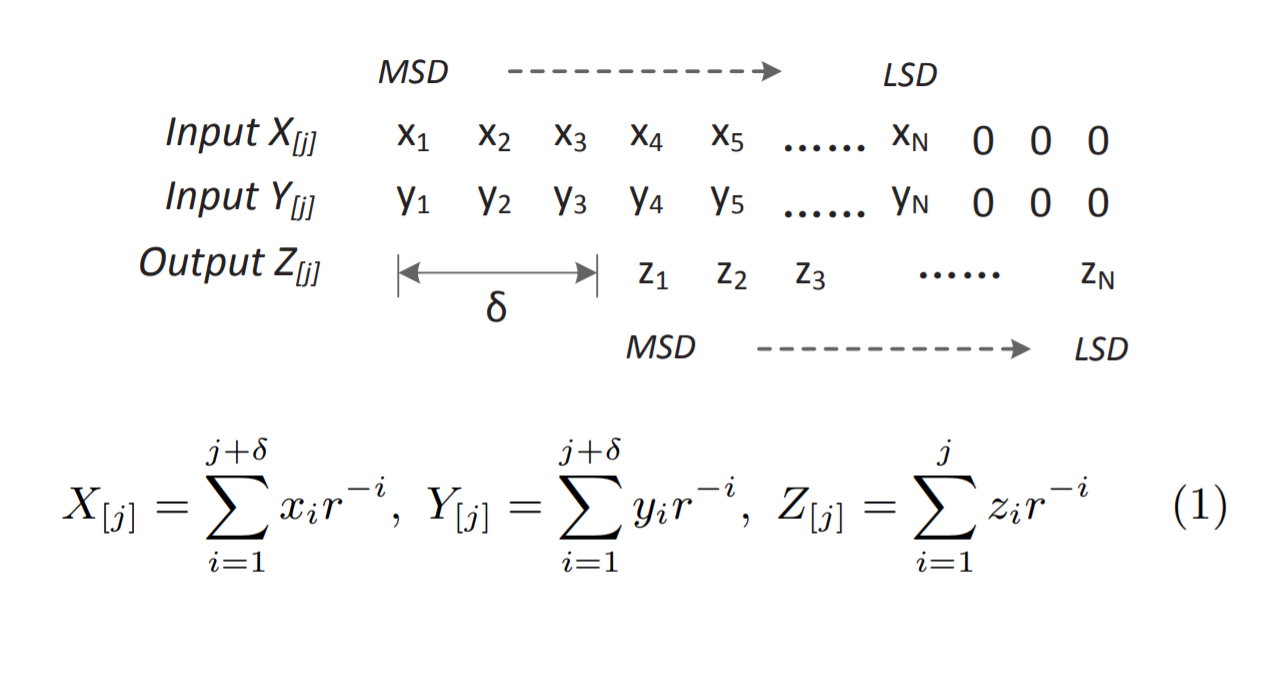
\includegraphics[scale=0.4]{f1.png}
       \caption{Data Flow in Digit-serial Online Arithmetic}
    \end{figure}
The other one is that online arithmetic uses redundant number representation\cite{c2}: when using radix-n sign-digit representation, the $i$ $^{th}$ digit of a number $x$,$x$ $^i$, lies in\{-\(n-1\),-\(n-2\),-\(n-3\),,.,0,..,\(n-3\),\(n-2\),\(n-1\)\}. And for each digit value, it will be represented by several bits in inputs. For instance, in radix-2, each digit will be in the range of -1,0,1, represented by two bits $x_+$, and $x_-$ and $x = x_+-x_-$.\cite{c4}.The basic radix-2 online calculators will be introduced here since project designs were made based on these modules and number representation for this is the one introduced before.
    
\subsubsection{Online Radix-2 Addition \cite{c2}}

Addition is one of the most basic arithmetic element and this can also be used in forming multiplier and divider. It uses full adders and sums up each digit of two adders from MSD to LSD as shown in figure 2(left). Tee first adder take charges of generating result of each digits and the second adder makes adjustments on digits value based on the condition that whether overflow appears or not.

Digits of output $z$ will appear after two clock cycles, which is known by online delay of this adder. when duplicating serial adder n times and removing registers, we get online digit-parallel adder. And it successfully removes online delay. There is a critical path between two full-adders\cite{c5}.The fixed critical path means that is a ripple-carry free addition which indicates that parallel adder is an adder having  its own running frequency independent to adder precision\cite{c6}.
         \begin{figure}[H]
       \centering
       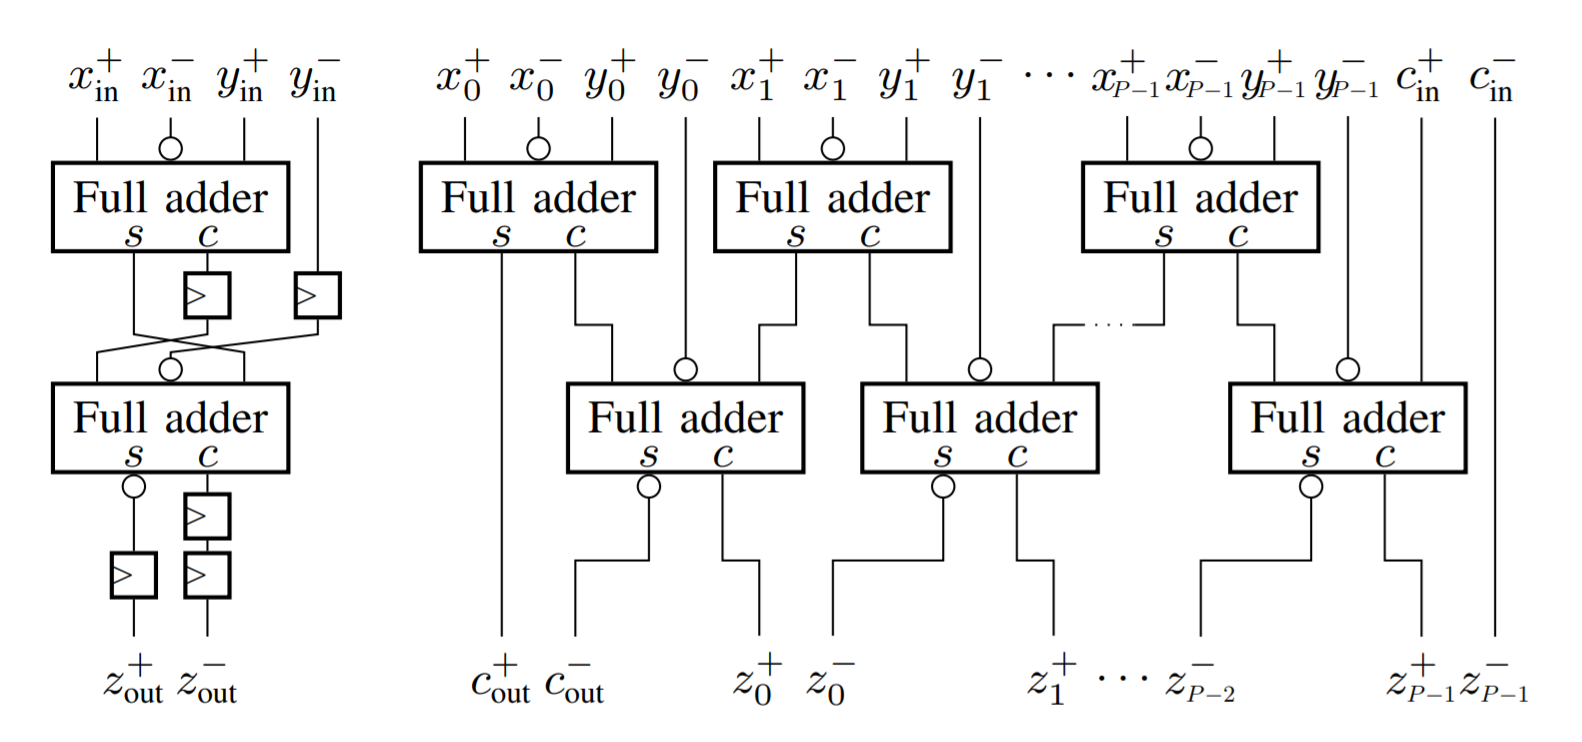
\includegraphics[scale=0.35]{f2.png}
       \caption{online serial and parallel adder}
    \end{figure}
    
The difference between structure of online adder and conventional adder is not that large since addition itself is a very simple computation. But the situation will be change in multiplication and division.
    
\subsubsection{Online Radix-2 Multiplication and Division}

Since in Online algorithm, the generated results of multiplication and division have same length of inputs. Thus there is an error tolerance between generated results and exact results. Assuming inputs have j digits. The error bound will bound will be 
\begin{gather}
    E = |f(x[j],y[j])-z[j]| < r^{-j}
\end{gather}

In order to limit error in this bound, we introduce a residual named $w[j]$ and bound the value of it with in a small range: |$w[j]|< \omega$:
\begin{gather}
    w[j] = r^j(f(x[j],y[j])-z[j])
\end{gather}

and we can prove $w[j+1]$ for multiplication and division are
\begin{gather}
    w[j+1] = rw[j]+(x[j]y_{j+1+\delta}+y[j+1]x_{j+1+\delta})r^{-\delta}-z[j+1]
\end{gather}
\begin{gather}
        w[j+1] = rw[j]+(x_{j+1+\delta}-z[j]y_{j+1+\delta})r^{-\delta}-y[j+1]z_{j+1}   
\end{gather}

We assign a variable named v[j] equals first two parts of w[j] for easy computation.

\begin{gather}
    v[j+1] = rw[j]+(x[j]y_{j+1+\delta}+y[j+1]x_{j+1+\delta})r^{-\delta}-z_{j+1}
\end{gather}

for multiplication
\begin{gather}
        v[j+1] = rw[j]+(x_{j+1+\delta}-z[j]y_{j+1+\delta})r^{-\delta}-y[j+1]z_{j+1}   
\end{gather}

for division.\\

The value for $z_{j+1}$ is determined selection function of $v[j]$ which guarantees w[j] keeps in bound, which is also controlled by online delay value set in system. for radix-2 system selection function of multiplier(SELM) and divider(SELD) is  :

\begin{gather}
        z_{j+1} = SELM(v[j]) = 
    \begin{cases}
        $1$,&   \frac{1}{2} \geq v[j] \leq \frac{7}{4}\\
        $0$,&   -\frac{1}{2} \geq v[j] \leq \frac{1}{4}\\
        $-1$,&  -2 \geq v[j] -\leq \frac{3}{4}\\
    \end{cases}
\end{gather} 

\begin{gather}
        z_{j+1} = SELD(v[j]) = 
    \begin{cases}
        $1$,&   \frac{1}{4} \geq v[j] \leq \frac{15}{8}\\
        $0$,&   -\frac{1}{4} \geq v[j] \leq \frac{1}{8}\\
        $-1$,&  -2 \geq v[j] -\leq \frac{1}{2}\\
    \end{cases}
\end{gather} 

The computation are shown blow:

        \begin{figure}[H]
       \centering
       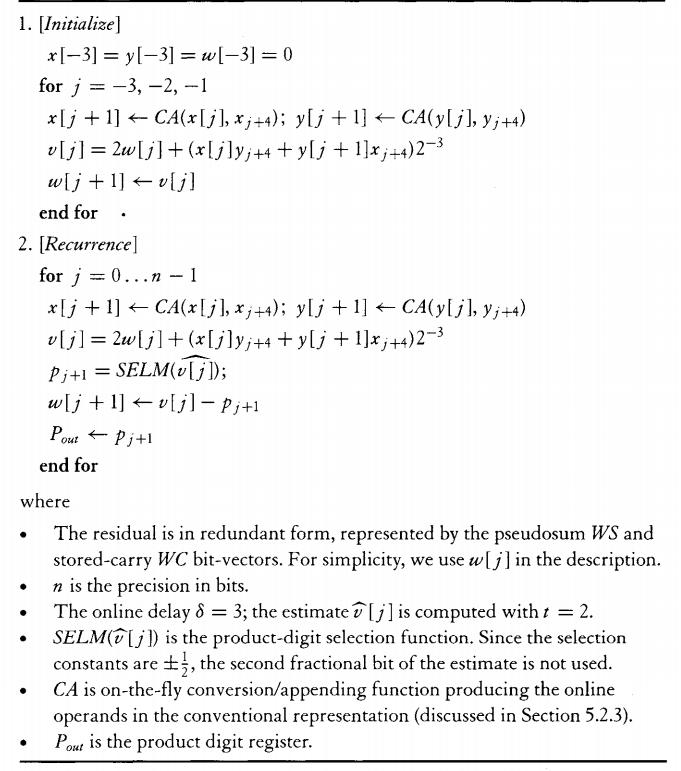
\includegraphics[scale=0.5]{multi_2_algo.PNG}
       \caption{online radix-2 multiplication algorithm }
    \end{figure}
    
    \begin{figure}[H]
       \centering
       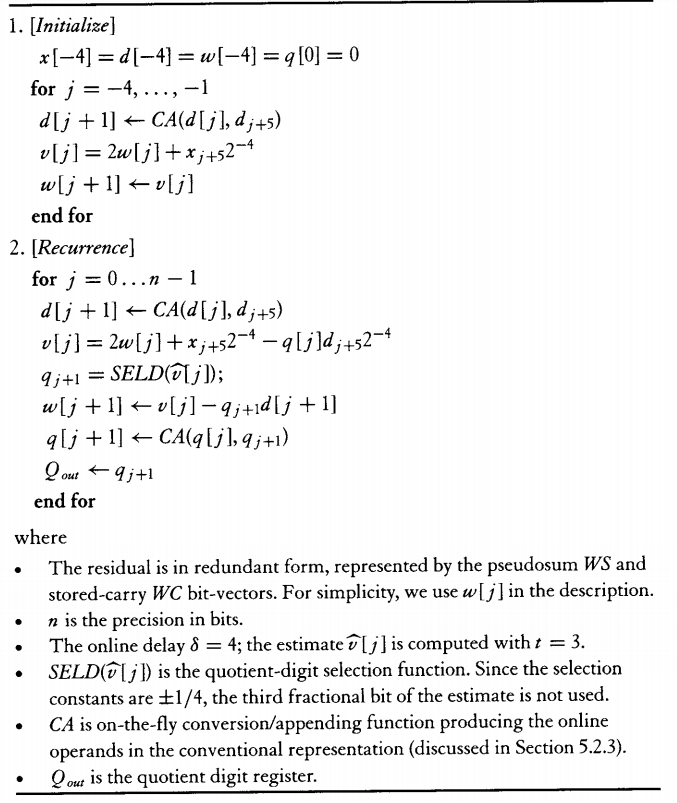
\includegraphics[scale=0.5]{divide_2_algo.PNG}
       \caption{online radix-2 division algorithm}
    \end{figure}


\subsection{Related Work to Online Algorithm}
There are lots of work has been done in the past. Parallel online operators  sacrifice hardware consumption to get higher processing speed and low system latency. A typical example is PasteUp system, a online radix-4 VLSI implementation arithmetic.\cite{c8}\cite{c9}
    
Recent researches also show that parallel online arithmetic is more graceful in overclocking since computation of online arithmetic start from MSD to LSD.In other word, it is more resistant to time error: LSD is the most vulnerable bit for error violation in online arithmetic while MSD is most vulnerable bit in traditional computation. \cite{c10}. Also,researchers put efforts on reducing hardware consumption especially area overhead. They introduce an online adder using four 6-input LUTs' resource optimizing built-in carry resource\cite{c10}.For some specific case, researchers decided to serial online operators which cost lower hardware resources. 

\subsection{Analysis of Online Arithmetic for High Radix Calculator Implementation Remains undeveloped}

Up to now, online algorithm has been well developed for radix-2 calculators with positive-negative number representation ($X = X^+-X^-$). However, there are very few materials discussing higher radix computation with online arithmetic and most of them are mainly analysing performance or optimization potential for radix-4 and 8. High-radix computation are very common in ASIC area. As it can largely reduce resources required for specific modules and accelerate processing speed for whole design. Based on large optimization potential proved of online algorithm in radix-2 calculation, there is large possibility that online algorithm can also accelerate higher radix-calculators. Motivated by this, project aims to find a general optimization solution for any  high-radix computation. !!!!!!!!!!!!!!!!!!!!!!!!!!!!!!!!



\section{Implementations}

\subsection{Environment Settings}

This project decided to use VHDL rather than Verilog to describe algorithm implemented hardware. First of all, in Verilog, all data types are predefined and each of them has a bit-level representation\cite{c10}. whereas VHDL is more verbose language describing hardware more detailed.It results in VHDL more often catches error missed in Verilog. As this project aims to describe hardware in gate level, it is beneficial to using a more detailed language. Secondly, there are some related projects available online writing by VHDL.It will be easier to compare performance with same language

The simulating FPGA hardware was chose to be Altera Cyclone V. Main reason behind it is that Cyclone V board is most available board in college. Thus it will be convenient to get access to simulate designs Also application installed in college computers is Quartus Prime with most modern version of Cyclone V installed in its library. 


\subsection{Modules Implementation}

For investigating the efficiency of higher-radix calculators, a new number representation method was introduced. Rather than using two bits representing $X^+$ and $X^-$ and number equals to
\begin{gather}
    X = X^+-X^-
\end{gather}
    Now $i+1$ bits 2's compliment signed numbers are used to represent in base-$2^{i}$ adder.
    
\begin{gather}
    X = -2^{i}X_{i+1}+2^{i-1}X_{i}+2^{i-2}X_{i-1}+....+X_1
\end{gather}
 With the represented range \{-$2^i$, $2^i$-1\}.  
 
 There are several benefits: firstly 2's compliment number representation is a more general method. It can easily adjust maximum represented range by adding or moving input bits. Secondly,2's compliment number addition is just binary addition, which will surely save used resources and accelerate processing speed. Moreover,its represented range starts from negative to positive number ,which ,meets the project requirement.Also, over-redundant-number-representing is also avoided. 
 
 One of the key features in this project designs is that all designs ports are flexible with radix-base and bandwidth. To achieve this, generic statement was introduced. It collects information from generic variables and generate required design based on inputs format.
 
 
         \begin{figure}[H]
       \centering
       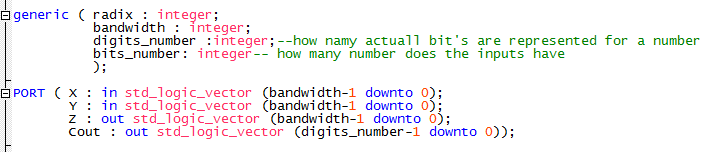
\includegraphics[scale=0.75]{code_generic.PNG}
       \caption{generic statement and ports setting}
    \end{figure}

\subsubsection{Adder}

Differ from the radix-2 online arithmetic, there are multiple bits used to represent a single digit. So the upper-line  full-adders are replaced with CA (carry-save adder) which consist of several full-adders. and a selection function.   
        \begin{figure}[H]
       \centering
       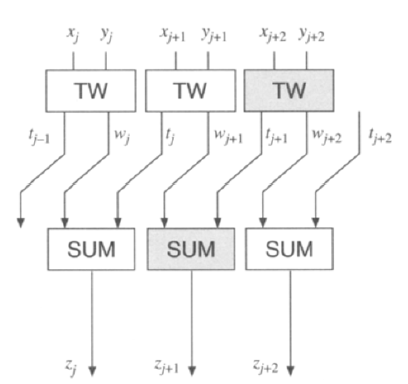
\includegraphics[scale=0.75]{adder_structure.png}
       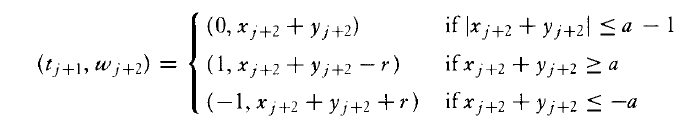
\includegraphics[scale=0.75]{SELA.png}
       \caption{online radix-2 addition \cite{c2}}
    \end{figure}
    
Noticeably, selection function is quite easy to be implemented. $t_{j+1}$ will be non-zero when overflow happens. And it signed equals to that of inputs.

        \begin{figure}[H]
       \centering
       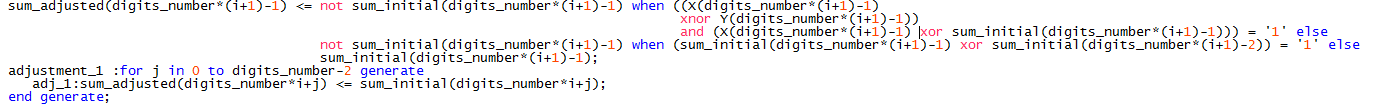
\includegraphics[width = 1\textwidth]{code_SELA.PNG}
       \caption{SELA code}
    \end{figure}
\subsubsection{Multiplier and Divider}

\paragraph{Selection Function}


The most conventional selection function is very complicated and allows many flexible choices,which is not
suitable for generating a general design of high-radix online calculation module. Selection by rounding  method \cite{c2} was used as selection in this project:
\begin{gather}
    Z_{j+1} = [v[j]+\frac{1}{2}]
\end{gather}
Moreover, this selection function is easy to be implemented since output bits can easily by taking integer part of $v[j]$ plus MSB of fraction part:
\begin{gather}
    Z_{j+1} = int(v[j])+[frac(v[j])]
\end{gather}

     \begin{figure}[H]
       \centering
       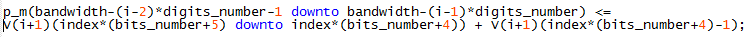
\includegraphics[scale=0.75]{code_SELM.PNG}
       \caption{SELM code}
    \end{figure}
    
\paragraph{Inner Multiplication}
!!!!!!!!!!!!!!!!!!!!!!
Both V[j]s in multiplication and division (eqn. 5,6) consist of multiplication of a single digits with the other input. This problem does not appear in radix-2 system since multiplication is only copy or inversion due to single digits length(equals to one). In this project, Basic conventional multiplication in "numeric\_std"was called to complete the inner multiplication.    

\section{Design Validation}

It is very necessary to validate output generated by online module. Only designs being able to produce correct results is worth being analysis their performance and resources requires. As for the design in this project, inputs' bandwidth and radix can theoretically go to infinity.Tome cost for validation increases dramatically when inputs' bandwidth or radix-base become a large number. It was decided that validation  module aims to test every possible inputs if inputs bandwidth is smaller than 20bits and random correctness was implemented when inputs bandwidth is higher.

\subsection{Validation code}

\subsubsection{Test With 20 Bits Or Lower Bandwidth Inputs}

There are steps of validating results:

{\large\bfseries Step1: generating valid inputs}

In order to test all possible inputs, the module will initialize inputs having all bits in value '0'. and they will increment by one after every single test being finished.  

{\large\bfseries Step2: computing correct output}

In redundant number representation,  a single value may have multiples of different digits value representation. Testing module transfers two inputs into conventional sign number and get the corresponding result in that format using "numeric\_std" library.

{\large\bfseries Step3: feeding inputs into online module}

{\large\bfseries Step4: converting generated result and comparing}

when computation of online calculation module is finished, test module transfer outputs into sign number format and 


\subsubsection{Test With Longer Inputs}

Compared with testing module, the only difference located in step1. Module will generate a random inputs by using function "range\_of\_rand".

\subsection{Correctness}

All simulation was done in ModelSim. With a correctness indicator bit C, it is clear that all design have past simulation test.
     \begin{figure}[H]
       \centering
       \includegraphics[scale=0.75]{sim_add_L.png}
       \includegraphics[scale=0.75]{sim_add_H.png}
       \caption{simulation result}
    \end{figure}
    
         \begin{figure}[H]
       \centering
       \includegraphics[scale=0.75]{sim_multi_L.png}
       \includegraphics[scale=0.75]{sim_multi_H.png}
       \caption{simulation result}
    \end{figure}
    
         \begin{figure}[H]
       \centering
       \includegraphics[scale=0.75]{sim_divide_L.png}
       \includegraphics[scale=0.75]{sim_divide_H.png}
       \caption{simulation result}
    \end{figure}
    
\section{performance analysis}  

\subsection{performance vs radix}

\subsection{performance comparison with online module and conventional modules }

\section{conclusion}


\section{Further Work}
\subsection{Generating Output for Arbitrary Function}
    Given that four basic operators perfectly work,the next step would be merging them together as a multi-functional module. For any given arbitrary function like Laplace transform or even complicated function,the module should able to separate the task into small basic tasks and finally generate result using a combination of 4 basic operators.
    
\subsection{Optimization Design for Specific FPGA}
    Even though final designed module should be runnable on any FPGAs.It is more likely to optimize module for a specific brand FPGA group or even a specific type of FPGA get higher efficiency. As FPGAs can be divided into two main groups : Altera and Xilinx series. Each series have their own IDE compiler and they have slight difference in hardware architectures, like different maximum pin toggle rates, RAM on-board distribution etc. Moreover,the choice may also be affected by possible environment which module actually being implemented.  
    
    
\begin{thebibliography}{99}

\bibitem{c1} M. D. Ercegovac, “On-line arithmetic: An overview,” in Proc. Annual
Technical Symp. Real time signal processing VII, 1984, pp. 86–93.

\bibitem{c2} M. D. Ercegovac and T. Lang, Digital arithmetic. Morgan Kaufmann,
2003.
\bibitem{c3} K. Shi, D. Boland, E. Stott, S. Bayliss, and G. A. Constantinides,
“Datapath synthesis for overclocking: Online arithmetic for latencyaccuracy trade-offs,” in Proc. DAC, June 2014.
\bibitem{c4} B. Parhami, “On the Implementation of Arithmetic Support Functions
for Generalized Signed-digit Number Systems,” IEEE Transactions on
Computers, vol. 42, no. 3, 1993.
\bibitem{c5} P. K.-G. Tu. On-line Arithmetic Algorithms for Efficient Implementation.
PhD thesis, University of California Los Angeles, 1990.
\bibitem{c6}  F. de Dinechin and B. Pasca, “Designing Custom Arithmetic Data Paths
with FloPoCo,” IEEE Design and Test of Computers, vol. 28, no. 4, 2011
\bibitem{c7}Yiren Zhao, J. Wickerson and G. A. Constantinides, "An efficient implementation of online arithmetic," 2016 International Conference on Field-Programmable Technology (FPT), Xi'an, 2016, pp. 69-76.
\bibitem{c8} R. Hartley and P. Corbett. Digit-serial processing techniques. IEEE
Transactions on Circuits and Systems, 37(6):707–719, June 1990.
\bibitem{c9}M. J. Irwin and R. M. Owens. Digit-pipelined arithmetic as illustrated
by the paste-up system: A tutorial. Computer, 20(4):61–73, Apr. 1987.
\bibitem{c10}K. Shi, D. Boland, E. Stott, S. Bayliss, and G. A. Constantinides.
Datapath synthesis for overclocking: Online arithmetic for latencyaccuracy trade-offs. DAC ’14, NY, USA, 2014. ACM.
\bibitem{c11}https://www.electronicdesign.com/what-s-difference-between/what-s-difference-between-vhdl-verilog-and-systemverilog
\end{thebibliography}

\end{document}